\documentclass[crop,tikz]{standalone}
\usetikzlibrary{decorations.pathreplacing}
\usetikzlibrary{arrows}
\begin{document}
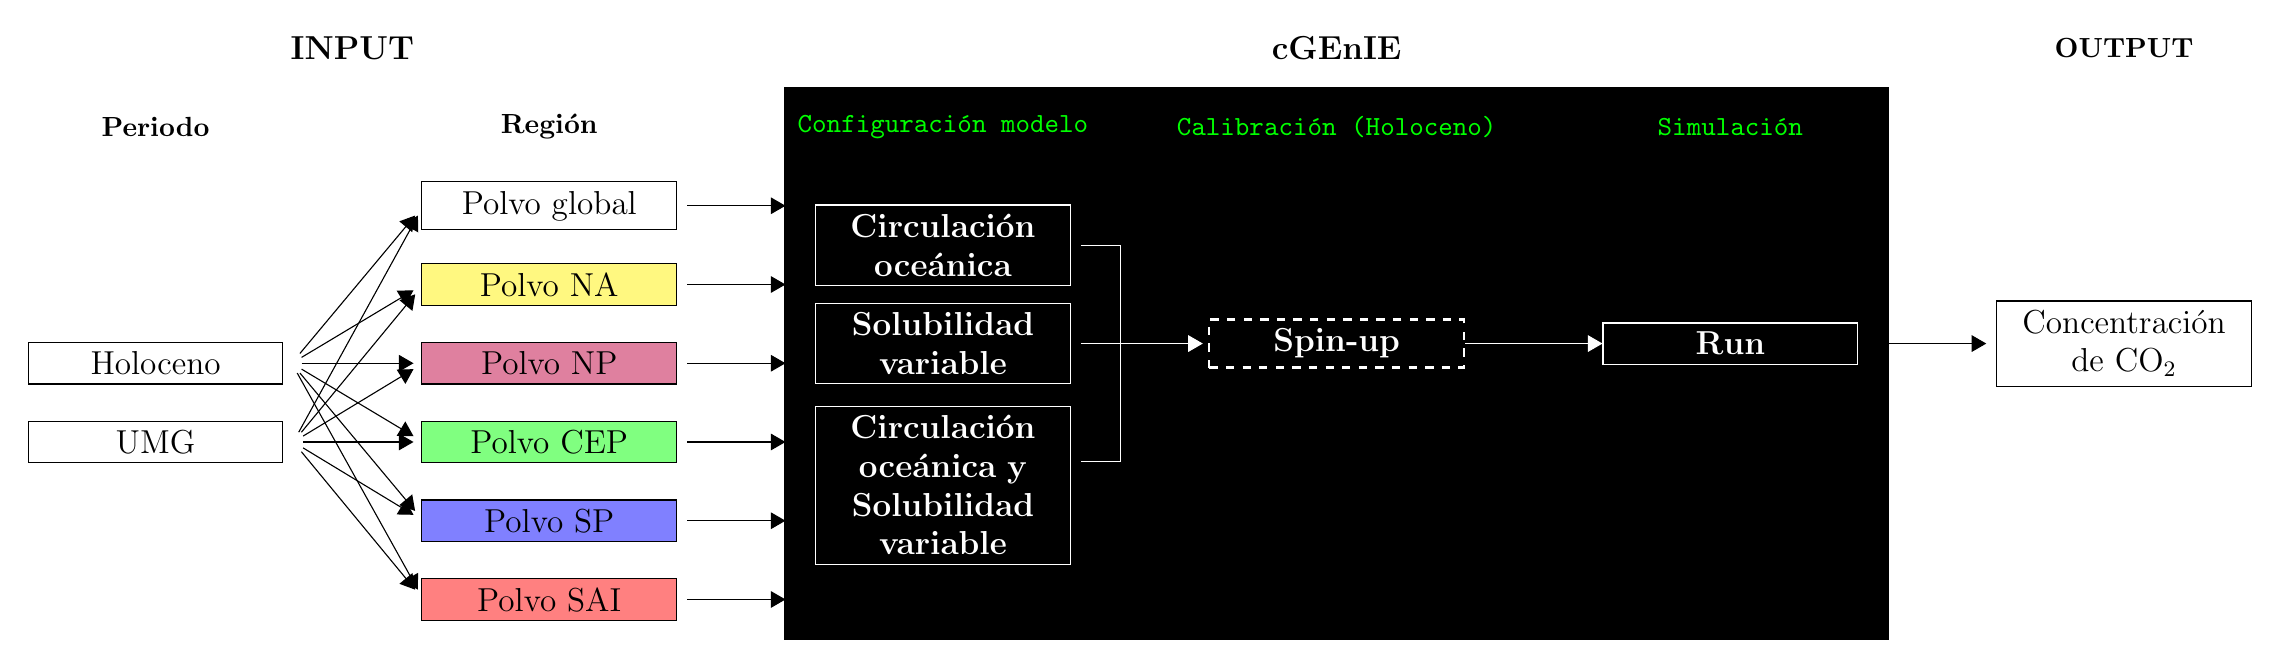
\begin{tikzpicture}
\tikzstyle{nodo texto}=[font=\large,draw,text width= 3cm,align=center]


%\node[nodo texto] at (-4.16,0.3) {Simulaciones };
%\draw[draw=none,fill=purple!50]  (3,2.75) rectangle (7,-0.75);
%\draw[draw=none,fill=red!50] (7,-1) rectangle (3,-2.5);

%\node[nodo texto] at (5,1.75) {Spin-up \\ (Nivel de polvo Holoceno)};
%\node[nodo texto] at (5,0.25) {Control \\ (Nivel de polvo Holoceno)};
%\node[nodo texto] at (5,0.5) {Run 1 \\ (Nivel de polvo 2)};
%\node[nodo texto] at (5,-1) {Run 2 \\ (Nivel de polvo 3)};
%\node[nodo texto] at (5,-1.75) {Run \\ (Nivel de polvo UMG)};


%\node[font=\Huge, sloped] at (5,-2.25) {$\vdots$};

% \draw [-triangle 60](1.75,1) node (v1) {} -- (3,1.75) node (v2) {};
% \draw [-triangle 60](v1) -- (3.25,-1.75) node (v4) {};
% \draw [-triangle 60](v1) -- (3.25,0.5) node (v5) {};
% \draw [-triangle 60](v1) -- (3.25,-1) node (v6) {};
% \draw [-triangle 60](v1) -- (3.25,-2.25);
% \draw [-triangle 60](v1) -- (3.25,-4) node (v7) {};
% \draw [dashed,-triangle 60](1.5,-0.5) node (v3) {} -- (v2);
% \draw [dashed,-triangle 60](v3) -- (v4);
% \draw [dashed,-triangle 60](v3) -- (v5);
% \draw [dashed,-triangle 60](v3) -- (v6);
% \draw [dashed,-triangle 60](v3) -- (3.25,-2);
% \draw [dashed,-triangle 60](v3) -- (v7);
% \draw [-triangle 60](-2.5,0.25) -- (-1.75,1);
% \draw [-triangle 60](-2.5,0.25) -- (-1.75,-0.5);
\draw[thick,fill]  (6.5,3) rectangle (20.5,-4);
\node[nodo texto] at (-1.5,-0.5) {Holoceno};
\node[nodo texto] at (-1.5,-1.5) {UMG};
\node[nodo texto]   at (3.5,1.5) {Polvo global};
\node[nodo texto,fill=yellow!50]  at (3.5,0.5) {Polvo NA};
\node[nodo texto,fill=purple!50]  at (3.5,-0.5) {Polvo NP};
\node[nodo texto,fill=green!50]  at (3.5,-1.5) {Polvo CEP};
\node[nodo texto,fill=blue!50]  at (3.5,-2.5) {Polvo SP};
\node[nodo texto,fill=red!50]  at (3.5,-3.5) {Polvo SAI};
\node[nodo texto,draw=white,text=white] at (8.5,1) {\bf Circulación oceánica };
%\node[nodo texto,draw=white,text=white] at (8.5,0) {\bf CO$_2$ libre};
\node[nodo texto,draw=white,text=white] at (8.5,-0.25) {\bf Solubilidad variable};
\node[nodo texto,draw=white,text=white] at (8.5,-2.05) {\bf Circulación oceánica y Solubilidad variable };
\node[nodo texto,thick,draw=white,text=white,dashed] (v10) at (13.5,-0.25) {\bf Spin-up};
\node[nodo texto,draw=white,text=white] (v11) at (18.5,-0.25) {\bf Run};
\node[nodo texto] at (23.5,-0.25) {Concentración de CO$_2$};
\node at (-1.5,2.5) {\bf Periodo};
\node at (3.5,2.5) {\bf Región};
\node[text=green] at (8.5,2.5) {\bf \texttt{Configuración modelo}};
\node[text=green] at (13.5,2.5) {\bf \texttt{Calibración (Holoceno)}};
\node[text=green] at (18.5,2.5) {\bf \texttt{Simulación}};
\node at (23.5,3.5) {\bf OUTPUT};
\node (v1) at (0.23,-0.5) {};
\node (v2) at (1.9,1.5) {};
\node (v3) at (1.9,0.5) {};
\node (v4) at (1.9,-0.5) {};
\node (v5) at (1.9,-1.5) {};
\node (v6) at (1.9,-2.5) {};
\node (v7) at (1.9,-3.5) {};
\draw [-triangle 60](v1) -- (v2);
\draw [-triangle 60](v1) -- (v3);
\draw [-triangle 60](v1) -- (v4);
\draw [-triangle 60](v1) -- (v5);
\draw [-triangle 60](v1) -- (v6);
\draw [-triangle 60](v1) -- (v7);
\node (v8) at (0.25,-1.5) {};
\draw [-triangle 60](v8) -- (v2);
\draw [-triangle 60] (v8) edge (v3);
\draw [-triangle 60] (v8) edge (v4);
\draw [-triangle 60] (v8) edge (v5);
\draw [-triangle 60] (v8) edge (v6);
\draw [-triangle 60] (v8) edge (v7);
%\draw [dashed] (1.5,3) rectangle (5.5,-4);
%\draw [dashed] (-3.5,3) rectangle (0.5,-4);
%\draw[dashed]  (21.5,3) rectangle (25.5,-4);
\draw [-triangle 60](5.25,1.5) -- (6.5,1.5);
\draw [-triangle 60](5.25,0.5) -- (6.5,0.5);
\draw [-triangle 60](5.25,-0.5) -- (6.5,-0.5);
\draw [-triangle 60](5.25,-1.5) -- (6.5,-1.5);
\draw [-triangle 60](5.25,-2.5) -- (6.5,-2.5);
\draw [-triangle 60](5.25,-3.5) -- (6.5,-3.5);
%\node (v9) at (12,-0.75) {};
%\draw [-triangle 60,draw=white](10.25,0.5) -- (v9);
%\draw [-triangle 60,draw=white](10.25,0) -- (v9);
%\draw [-triangle 60,draw=white](10.25,-0.75) -- (v9);
%\draw [-triangle 60,draw=white](10.25,-2.25) -- (v9);
\draw [-triangle 60,draw=white] (v10) -- (v11);
\draw [-triangle 60](20.5,-0.25) -- (21.75,-0.25);
\node at (13.5,3.5) {\bf \large cGEnIE};
%\draw [thick,draw=white,dashed] (11.5,3) rectangle (15.5,-4);
%\draw [draw=white,-triangle 60](10.25,0.5) -- (11.8,0.5);
\draw [draw=white,-triangle 60](10.25,-0.25) -- (11.8,-0.25);
%\draw [draw=white,-triangle 60](10.25,-2.25) -- (11.8,-2.25);
\draw [white](10.25,1) -- (10.75,1) -- (10.75,-1.75) -- (10.25,-1.75);
\node at (1,3.5) {\bf \large INPUT};
\end{tikzpicture}
\end{document}
    